\chapter{Analisi ammortizzata}

\index{analisi ammortizzata}

La complessità computazionale di un algoritmo
è spesso facile da analizzare, 
esaminando la struttura dell'algoritmo:
quanti cicli contiene e quante volte 
questi cicli sono eseguiti.
Comunque non sempre un'analisi diretta
da una stima significativa dell'efficienza di un algoritmo.

L'\key{analisi ammortizzata} può essere usata per analizzare
algoritmi che contengono operazioni la 
cui complessità varia nelle varie esecuzioni.
L'idea è di stimare il tempo totale usato
da tutte le operazioni eseguite dall'algoritmo,
al posto di concentrarsi sulle singole operazioni.

\section{Metodo dei due puntatori}

\index{metodo dei due puntatori}

Nel \key{metodo dei due puntatori},
vengono utilizzati due puntatori, o indici, 
per iterare attraverso i valori di un array.
Entrambi i puntatori possono muoversi in una direzione soltanto,
il chè assicura che l'algoritmo sarà molto efficiente.
Adesso si discuteranno due problemi in cui
può essere utilizzato questo metodo.

\subsubsection{Somma di un sottovettore}

Come primo esempio,
si consideri un problema dove,
dato un vettore composto da $n$ interi positivi
e una somma obiettivo $x$,
si voglia trovare un sottovettore la cui somma sia
esattamente $x$, oppure comunicare che questa cosa non è possibile.

Per esempio, l'array
\begin{center}
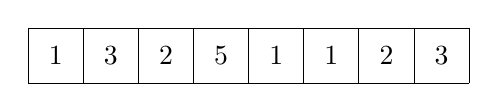
\begin{tikzpicture}[scale=0.7]
\draw (0,0) grid (8,1);

\node at (0.5,0.5) {$1$};
\node at (1.5,0.5) {$3$};
\node at (2.5,0.5) {$2$};
\node at (3.5,0.5) {$5$};
\node at (4.5,0.5) {$1$};
\node at (5.5,0.5) {$1$};
\node at (6.5,0.5) {$2$};
\node at (7.5,0.5) {$3$};
\end{tikzpicture}
\end{center}
contiene un sottovettore la cui somma è 8:
\begin{center}
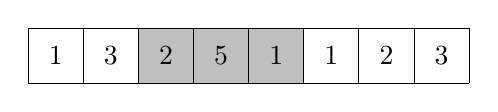
\begin{tikzpicture}[scale=0.7]
\fill[color=lightgray] (2,0) rectangle (5,1);
\draw (0,0) grid (8,1);

\node at (0.5,0.5) {$1$};
\node at (1.5,0.5) {$3$};
\node at (2.5,0.5) {$2$};
\node at (3.5,0.5) {$5$};
\node at (4.5,0.5) {$1$};
\node at (5.5,0.5) {$1$};
\node at (6.5,0.5) {$2$};
\node at (7.5,0.5) {$3$};
\end{tikzpicture}
\end{center}

Questo problema può essere risolto in tempo
$O(n)$ usando il metodo dei due puntatori.
L'idea è quella di avere un puntatore al primo e 
l'altro all'ultimo elemento del sottovettore cercato.
A ogni passaggio, il puntatore di sinistra si muoverà 
di un passo a destra e il puntatore destro si muoverà a destra
fino a quando la somma del sottovettore risultante sia al massimo $x$.
Se la somma diventa esattamente $x$,
allora è stata trovata una soluzione.

Come esempio si consideri questo array e 
la somma obiettivo sia $x=8$:
\begin{center}
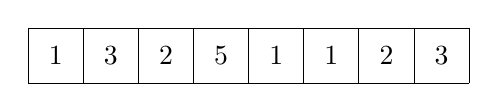
\begin{tikzpicture}[scale=0.7]
\draw (0,0) grid (8,1);

\node at (0.5,0.5) {$1$};
\node at (1.5,0.5) {$3$};
\node at (2.5,0.5) {$2$};
\node at (3.5,0.5) {$5$};
\node at (4.5,0.5) {$1$};
\node at (5.5,0.5) {$1$};
\node at (6.5,0.5) {$2$};
\node at (7.5,0.5) {$3$};
\end{tikzpicture}
\end{center}

All'inizio il sottovettore contiene i valori
1, 3 e 2, la cui somma è 6 (il 5 non viene incluso adesso
perchè porterebbe la somma a un valore maggiore di 8):

\begin{center}
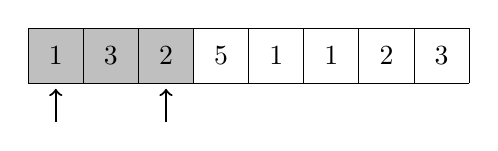
\begin{tikzpicture}[scale=0.7]
\fill[color=lightgray] (0,0) rectangle (3,1);
\draw (0,0) grid (8,1);

\node at (0.5,0.5) {$1$};
\node at (1.5,0.5) {$3$};
\node at (2.5,0.5) {$2$};
\node at (3.5,0.5) {$5$};
\node at (4.5,0.5) {$1$};
\node at (5.5,0.5) {$1$};
\node at (6.5,0.5) {$2$};
\node at (7.5,0.5) {$3$};

\draw[thick,->] (0.5,-0.7) -- (0.5,-0.1);
\draw[thick,->] (2.5,-0.7) -- (2.5,-0.1);
\end{tikzpicture}
\end{center}

Poi il puntatore di sinistra si muove di una posizione a destra
e ancora il puntatore destro sta fermo, altrimenti la somma
eccederebbe il valore di $x$.

\begin{center}
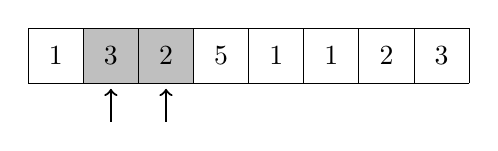
\begin{tikzpicture}[scale=0.7]
\fill[color=lightgray] (1,0) rectangle (3,1);
\draw (0,0) grid (8,1);

\node at (0.5,0.5) {$1$};
\node at (1.5,0.5) {$3$};
\node at (2.5,0.5) {$2$};
\node at (3.5,0.5) {$5$};
\node at (4.5,0.5) {$1$};
\node at (5.5,0.5) {$1$};
\node at (6.5,0.5) {$2$};
\node at (7.5,0.5) {$3$};

\draw[thick,->] (1.5,-0.7) -- (1.5,-0.1);
\draw[thick,->] (2.5,-0.7) -- (2.5,-0.1);
\end{tikzpicture}
\end{center}

Il puntatore di sinistra si muove ancora di un passo, 
e questa volta il puntatore di destra si muove di 2 passi
a destra.
Siccome adesso la somma è esattamente 8 ($2+5+1$),
la soluzione cercata è stata trovata.

\begin{center}
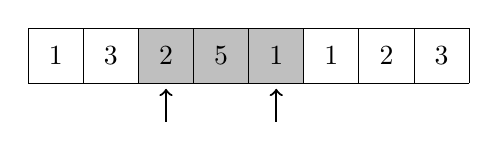
\begin{tikzpicture}[scale=0.7]
\fill[color=lightgray] (2,0) rectangle (5,1);
\draw (0,0) grid (8,1);

\node at (0.5,0.5) {$1$};
\node at (1.5,0.5) {$3$};
\node at (2.5,0.5) {$2$};
\node at (3.5,0.5) {$5$};
\node at (4.5,0.5) {$1$};
\node at (5.5,0.5) {$1$};
\node at (6.5,0.5) {$2$};
\node at (7.5,0.5) {$3$};

\draw[thick,->] (2.5,-0.7) -- (2.5,-0.1);
\draw[thick,->] (4.5,-0.7) -- (4.5,-0.1);
\end{tikzpicture}
\end{center}

Il tempo di esecuzione di questo algoritmo dipende
dal numero di spostamenti che compie il puntatore
di destra a ogni passaggio.
Nonostante non ci sia un limite superiore significativo 
al numero di spostamenti che può compiere a ogni singolo
passaggio, si può comunque vedere che il puntatore farà al 
massimo \emph{un totale di}
$O(n)$ passaggi durante l'algoritmo,
poichè si muove sempre e solo a destra.

Poichè sia il puntatore di sinistra che quello di destra
si muovono di $O(n)$ passi durante l'esecuzione dell'algoritmo,
la complessità computazionale è di tipo $O(n)$.

\subsubsection{2SUM problem}

\index{2SUM problem}

Un altro problema che può essere risolto con 
il metodo dei due puntatori è il seguente, 
conosciuto anche con il nome di  \key{2SUM problem}:
dato un array di $n$ numeri e una somma obiettivo $x$,
trovare due elementi dell'array tali che la loro
somma sia esattamente $x$ oppure indicare
che non è possibile.
Per risolvere questo problema è prima
necessario ordinare l'array in modo crescente.
Successivamente si potrà iterare attraverso l'array
usando sempre due puntatori.
Il puntatore di sinistra partirà alla prima posizione
e si muoverà di una posizione verso destra ad ogni
passaggio dell'algoritmo.
Il puntatore di destra partirà invece in ultima posizione
e si muoverà verso sinistra fino a quando la somma degli 
elementi indicati dai due puntatori non
sarà al massimo $x$.
Se la somma dovesse diventare esattamente $x$
è stata trovata la soluzione.

Si consideri ad esempio il seguente array e 
che la somma obiettivo sia $x=12$:
\begin{center}
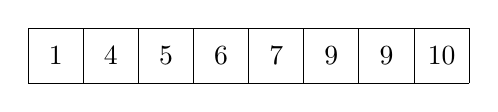
\begin{tikzpicture}[scale=0.7]
\draw (0,0) grid (8,1);

\node at (0.5,0.5) {$1$};
\node at (1.5,0.5) {$4$};
\node at (2.5,0.5) {$5$};
\node at (3.5,0.5) {$6$};
\node at (4.5,0.5) {$7$};
\node at (5.5,0.5) {$9$};
\node at (6.5,0.5) {$9$};
\node at (7.5,0.5) {$10$};
\end{tikzpicture}
\end{center}

Le posizioni iniziali dei puntatori sono 
come descritto sopra e la somma è $1+10=11$
che è più piccolo di $x$.

\begin{center}
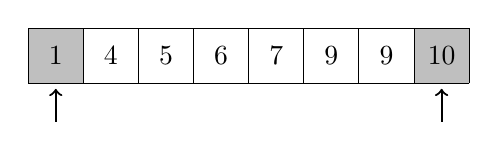
\begin{tikzpicture}[scale=0.7]
\fill[color=lightgray] (0,0) rectangle (1,1);
\fill[color=lightgray] (7,0) rectangle (8,1);
\draw (0,0) grid (8,1);

\node at (0.5,0.5) {$1$};
\node at (1.5,0.5) {$4$};
\node at (2.5,0.5) {$5$};
\node at (3.5,0.5) {$6$};
\node at (4.5,0.5) {$7$};
\node at (5.5,0.5) {$9$};
\node at (6.5,0.5) {$9$};
\node at (7.5,0.5) {$10$};

\draw[thick,->] (0.5,-0.7) -- (0.5,-0.1);
\draw[thick,->] (7.5,-0.7) -- (7.5,-0.1);
\end{tikzpicture}
\end{center}

Il puntatore di sinistra si muove di una posizione a destra,
mentre quello di destra si muove di tre passi a sinistra,
e la somma diventa $4+7=11$.

\begin{center}
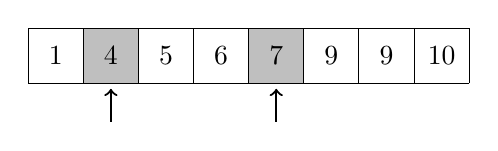
\begin{tikzpicture}[scale=0.7]
\fill[color=lightgray] (1,0) rectangle (2,1);
\fill[color=lightgray] (4,0) rectangle (5,1);
\draw (0,0) grid (8,1);

\node at (0.5,0.5) {$1$};
\node at (1.5,0.5) {$4$};
\node at (2.5,0.5) {$5$};
\node at (3.5,0.5) {$6$};
\node at (4.5,0.5) {$7$};
\node at (5.5,0.5) {$9$};
\node at (6.5,0.5) {$9$};
\node at (7.5,0.5) {$10$};

\draw[thick,->] (1.5,-0.7) -- (1.5,-0.1);
\draw[thick,->] (4.5,-0.7) -- (4.5,-0.1);
\end{tikzpicture}
\end{center}

Al passaggio successivo il puntatore di sinistra si muove di un ulteriore
passo verso destra e il puntatore di destra non si muove poichè 
$5+7=12$ e quindi è stata trovata la soluzione.

\begin{center}
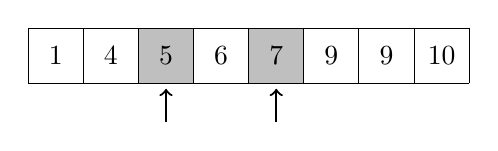
\begin{tikzpicture}[scale=0.7]
\fill[color=lightgray] (2,0) rectangle (3,1);
\fill[color=lightgray] (4,0) rectangle (5,1);
\draw (0,0) grid (8,1);

\node at (0.5,0.5) {$1$};
\node at (1.5,0.5) {$4$};
\node at (2.5,0.5) {$5$};
\node at (3.5,0.5) {$6$};
\node at (4.5,0.5) {$7$};
\node at (5.5,0.5) {$9$};
\node at (6.5,0.5) {$9$};
\node at (7.5,0.5) {$10$};

\draw[thick,->] (2.5,-0.7) -- (2.5,-0.1);
\draw[thick,->] (4.5,-0.7) -- (4.5,-0.1);
\end{tikzpicture}
\end{center}

Il tempo di esecuzione di questo algoritmo è quindi
$O(n \log n)$, poichè l'ordinamento iniziale costa $O(n \log n)$ e
poi i due puntatori si muovono di $O(n)$ posizioni.

Si può notare che è possibile risolvere il problema in un altro
modo, sempre a un costo di $O(n \log n)$ usando la ricerca binaria.
Seguendo quest'idea, si itera attraverso il vettore ordinato e, per ogni elemento, si cerca
un altro valore che sommato a quello corrente dia somma $x$.
Questo può essere fatto effettuando $n$ ricerche binarie,
ognuna delle quali costa $O(\log n)$.

\index{3SUM problem}
Un problema più complesso è quello chiamato
\key{3SUM problem}, che chiede di trovare \emph{tre} elementi del vettore la 
cui somma sia esattamente $x$.
Usando l'idea risolutiva dell'algoritmo precedente,
questo problema può essere risolto con costo $O(n^2)$\footnote{
Per molto tempo si è pensato che risolvere questo problema
con un costo inferiore a $O(n^2)$ non fosse possibile.
Invece nel 2014 si è scoperto \cite{gro14}
che si può fare di meglio.}. Sei in grado di vedere come?

\section{Nearest smaller elements}
\label{sec:nearest_smaller_elements}

\index{nearest smaller elements}

L'analisi ammortizzata è utilizzata spesso per
stimare il numero di operazioni 
effettuate su una struttura dati.
Le operazioni potrebbero anche essere distribuite in maniera differente,
con la maggior parte di esse concentrate in
una certa fase dell'algoritmo,
ma resta possibile trovare il numero totale di operazioni, che
rimane comunque limitato.

Come esempio si consideri il problema 
di trovare, per ogni elemento di un array,
il \key{nearest smaller element}, cioè
il primo elemento più piccolo che precede 
un certo elemento nell'array. Più formalmente,
dato l'elemento $v_{i}$, bisogna trovare l'elemento
$v_{j}$ con $0 \leq j<i$, tale che $v_{j} < v_{i}$ e che abbia l'indice $j$
più grande tra tutti quelli che soddisfano la condizione precedente.
Nel caso tale elemento non esistesse,
l'algoritmo dovrà riportare questa condizione.
Si vedrà adesso come risolvere in maniera
efficiente questo problema utilizzando una pila.

Si inizia iterando sul vettore da sinistra a destra
e mantenendo una pila degli elementi dell'array.
Per ogni posizione verranno rimossi tutti gli elementi
in cima alla pila, fino a quando verrà trovato un
elemento minore dell'elemento corrente dell'array,
oppure fino a quando la pila non sarà vuota.
Poi si procede indicando l'elemento in cima alla
pila come quello cercato, cioè il \emph{nearest smaller element},
oppure indicando che non esiste se la pila fosse vuota.
Come ultimo passo l'elemento corrente verrà inserito nella pila. 

Si consideri ad esempio il seguente array:
\begin{center}
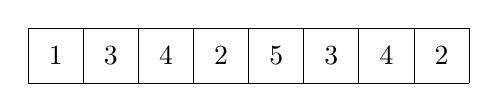
\begin{tikzpicture}[scale=0.7]
\draw (0,0) grid (8,1);

\node at (0.5,0.5) {$1$};
\node at (1.5,0.5) {$3$};
\node at (2.5,0.5) {$4$};
\node at (3.5,0.5) {$2$};
\node at (4.5,0.5) {$5$};
\node at (5.5,0.5) {$3$};
\node at (6.5,0.5) {$4$};
\node at (7.5,0.5) {$2$};
\end{tikzpicture}
\end{center}

Inizialmente gli elementi 1, 3 e 4 verranno aggiunti alla pila,
poichè ogni elemento è maggiore del precedente.
Quindi il \emph{nearest smaller element} di 4 è 3 e quello di 3 è 1.
\begin{center}
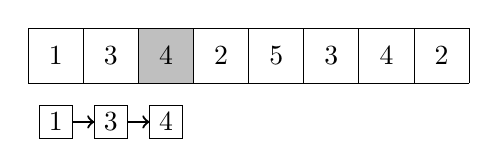
\begin{tikzpicture}[scale=0.7]
\fill[color=lightgray] (2,0) rectangle (3,1);
\draw (0,0) grid (8,1);

\node at (0.5,0.5) {$1$};
\node at (1.5,0.5) {$3$};
\node at (2.5,0.5) {$4$};
\node at (3.5,0.5) {$2$};
\node at (4.5,0.5) {$5$};
\node at (5.5,0.5) {$3$};
\node at (6.5,0.5) {$4$};
\node at (7.5,0.5) {$2$};

\draw (0.2,0.2-1.2) rectangle (0.8,0.8-1.2);
\draw (1.2,0.2-1.2) rectangle (1.8,0.8-1.2);
\draw (2.2,0.2-1.2) rectangle (2.8,0.8-1.2);

\node at (0.5,0.5-1.2) {$1$};
\node at (1.5,0.5-1.2) {$3$};
\node at (2.5,0.5-1.2) {$4$};

\draw[->,thick] (0.8,0.5-1.2) -- (1.2,0.5-1.2);
\draw[->,thick] (1.8,0.5-1.2) -- (2.2,0.5-1.2);
\end{tikzpicture}
\end{center}

A questo punto il 2 diventa il nuovo elemento corrente
ed è anche più piccolo dei primi due elementi in cima
alla pila, il 3 e il 4, quindi essi saranno rimossi dalla pila.
Il \emph{nearest smaller element} di 2 sarà quindi 1, l'elemento 
in cima alla pila, e il 2 verrà successivamente aggiunto alla pila.
\begin{center}
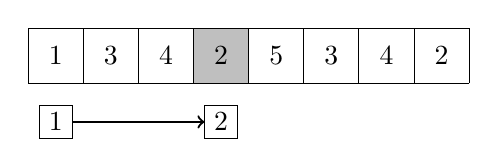
\begin{tikzpicture}[scale=0.7]
\fill[color=lightgray] (3,0) rectangle (4,1);
\draw (0,0) grid (8,1);

\node at (0.5,0.5) {$1$};
\node at (1.5,0.5) {$3$};
\node at (2.5,0.5) {$4$};
\node at (3.5,0.5) {$2$};
\node at (4.5,0.5) {$5$};
\node at (5.5,0.5) {$3$};
\node at (6.5,0.5) {$4$};
\node at (7.5,0.5) {$2$};

\draw (0.2,0.2-1.2) rectangle (0.8,0.8-1.2);
\draw (3.2,0.2-1.2) rectangle (3.8,0.8-1.2);

\node at (0.5,0.5-1.2) {$1$};
\node at (3.5,0.5-1.2) {$2$};

\draw[->,thick] (0.8,0.5-1.2) -- (3.2,0.5-1.2);
\end{tikzpicture}
\end{center}

Poi l'elemento 5, che è maggiore di 2,
verrà aggiunto alla pila e il suo \emph{nearest smaller element}
risulterà il numero 2:
\begin{center}
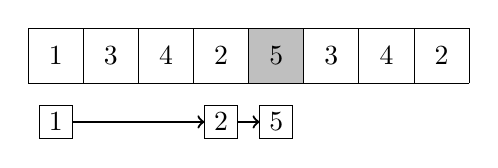
\begin{tikzpicture}[scale=0.7]
\fill[color=lightgray] (4,0) rectangle (5,1);
\draw (0,0) grid (8,1);

\node at (0.5,0.5) {$1$};
\node at (1.5,0.5) {$3$};
\node at (2.5,0.5) {$4$};
\node at (3.5,0.5) {$2$};
\node at (4.5,0.5) {$5$};
\node at (5.5,0.5) {$3$};
\node at (6.5,0.5) {$4$};
\node at (7.5,0.5) {$2$};

\draw (0.2,0.2-1.2) rectangle (0.8,0.8-1.2);
\draw (3.2,0.2-1.2) rectangle (3.8,0.8-1.2);
\draw (4.2,0.2-1.2) rectangle (4.8,0.8-1.2);

\node at (0.5,0.5-1.2) {$1$};
\node at (3.5,0.5-1.2) {$2$};
\node at (4.5,0.5-1.2) {$5$};

\draw[->,thick] (0.8,0.5-1.2) -- (3.2,0.5-1.2);
\draw[->,thick] (3.8,0.5-1.2) -- (4.2,0.5-1.2);
\end{tikzpicture}
\end{center}

Continuando in questo modo il 5 verrà rimosso dalla pila e
verranno aggiunti il 3 e il 4:
\begin{center}
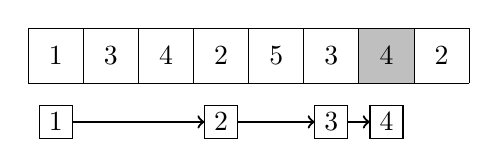
\begin{tikzpicture}[scale=0.7]
\fill[color=lightgray] (6,0) rectangle (7,1);
\draw (0,0) grid (8,1);

\node at (0.5,0.5) {$1$};
\node at (1.5,0.5) {$3$};
\node at (2.5,0.5) {$4$};
\node at (3.5,0.5) {$2$};
\node at (4.5,0.5) {$5$};
\node at (5.5,0.5) {$3$};
\node at (6.5,0.5) {$4$};
\node at (7.5,0.5) {$2$};

\draw (0.2,0.2-1.2) rectangle (0.8,0.8-1.2);
\draw (3.2,0.2-1.2) rectangle (3.8,0.8-1.2);
\draw (5.2,0.2-1.2) rectangle (5.8,0.8-1.2);
\draw (6.2,0.2-1.2) rectangle (6.8,0.8-1.2);

\node at (0.5,0.5-1.2) {$1$};
\node at (3.5,0.5-1.2) {$2$};
\node at (5.5,0.5-1.2) {$3$};
\node at (6.5,0.5-1.2) {$4$};

\draw[->,thick] (0.8,0.5-1.2) -- (3.2,0.5-1.2);
\draw[->,thick] (3.8,0.5-1.2) -- (5.2,0.5-1.2);
\draw[->,thick] (5.8,0.5-1.2) -- (6.2,0.5-1.2);
\end{tikzpicture}
\end{center}

Infine verranno rimossi dalla pila tutti gli 
elementi tranne l'1 e il 2 verrà inserito nella pila:

\begin{center}
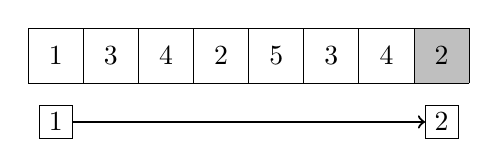
\begin{tikzpicture}[scale=0.7]
\fill[color=lightgray] (7,0) rectangle (8,1);
\draw (0,0) grid (8,1);

\node at (0.5,0.5) {$1$};
\node at (1.5,0.5) {$3$};
\node at (2.5,0.5) {$4$};
\node at (3.5,0.5) {$2$};
\node at (4.5,0.5) {$5$};
\node at (5.5,0.5) {$3$};
\node at (6.5,0.5) {$4$};
\node at (7.5,0.5) {$2$};

\draw (0.2,0.2-1.2) rectangle (0.8,0.8-1.2);
\draw (7.2,0.2-1.2) rectangle (7.8,0.8-1.2);

\node at (0.5,0.5-1.2) {$1$};
\node at (7.5,0.5-1.2) {$2$};

\draw[->,thick] (0.8,0.5-1.2) -- (7.2,0.5-1.2);
\end{tikzpicture}
\end{center}

L'efficienza di questo algoritmo dipende 
dal numero totale di operazioni effettuate sulla pila.
Se l'elemento corrente è più grande dell'elemento
in cima alla pila verrà fatto solo un inserimento,
che ovviamente è efficiente.
Se invece, come capiterà un certo numero di volte nei casi medi,
dovranno essere rimossi gli elementi più piccoli 
di quello corrente, allora questo richiederà più tempo.
Comunque ogni elemento verrà inserito \emph{esattamente una volta} e rimosso
\emph{esattamente una volta} e quindi causerà $O(1)$ operazioni sulla pila,
portando quindi l'algoritmo ad avere complessità 
$O(n)$.

\section{Sliding window minimum}

\index{sliding window}
\index{sliding window minimum}

Una \key{sliding window} (finestra mobile) è un sottovettore di lunghezza costante
che si muove da sinistra a destra all'interno di un vettore.
Per ogni posizione della finestra mobile
si vuole calcolare un qualche genere di informazione
che riguarda gli elementi contenuti.
In questa sezione ci si focalizzerà
sul problema di trovare il minimo contenuto
in ogni finestra mobile, detto anche problema
\key{sliding window minimum}.

Questo problema può essere risolto usando
un'idea simile a quella utilizzata per risolvere il 
problema del paragrafo \ref{sec:nearest_smaller_elements}.

Stavolta si utilizzerà una coda,
dove ogni elemento è più grande dell'elemento che lo precede,
in modo che il primo elemento sia sempre il più piccolo
tra quelli presenti nella finestra mobile.
A ogni movimento successivo della finestra mobile,
verranno rimossi tutti gli elementi in fondo alla coda 
fino a quando non se ne troverà uno minore di quello
nuovo presente nella finestra mobile o fino a quando 
la coda diventerà vuota.

Verrà anche rimosso il primo elemento della coda,
poichè sarà "slittato" fuori dalla finestra mobile.
Infine il nuovo elemento verrà aggiunto alla fine 
della coda.

Si consideri ad esempio il seguente vettore:

\begin{center}
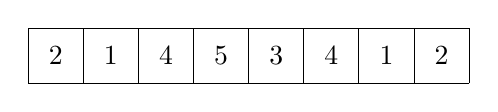
\begin{tikzpicture}[scale=0.7]
\draw (0,0) grid (8,1);

\node at (0.5,0.5) {$2$};
\node at (1.5,0.5) {$1$};
\node at (2.5,0.5) {$4$};
\node at (3.5,0.5) {$5$};
\node at (4.5,0.5) {$3$};
\node at (5.5,0.5) {$4$};
\node at (6.5,0.5) {$1$};
\node at (7.5,0.5) {$2$};
\end{tikzpicture}
\end{center}

Si supponga che la dimensione della finestra mobile sia 4.
Alla posizione di partenza della finestra, l'elemento 
più piccolo vale 1:
\begin{center}
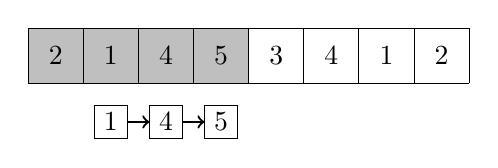
\begin{tikzpicture}[scale=0.7]
\fill[color=lightgray] (0,0) rectangle (4,1);
\draw (0,0) grid (8,1);

\node at (0.5,0.5) {$2$};
\node at (1.5,0.5) {$1$};
\node at (2.5,0.5) {$4$};
\node at (3.5,0.5) {$5$};
\node at (4.5,0.5) {$3$};
\node at (5.5,0.5) {$4$};
\node at (6.5,0.5) {$1$};
\node at (7.5,0.5) {$2$};

\draw (1.2,0.2-1.2) rectangle (1.8,0.8-1.2);
\draw (2.2,0.2-1.2) rectangle (2.8,0.8-1.2);
\draw (3.2,0.2-1.2) rectangle (3.8,0.8-1.2);

\node at (1.5,0.5-1.2) {$1$};
\node at (2.5,0.5-1.2) {$4$};
\node at (3.5,0.5-1.2) {$5$};

\draw[->,thick] (1.8,0.5-1.2) -- (2.2,0.5-1.2);
\draw[->,thick] (2.8,0.5-1.2) -- (3.2,0.5-1.2);
\end{tikzpicture}
\end{center}

Poi la finestra si sposta di un passo a destra.
Il nuovo elemento 3 è più piccolo degli elementi
4 e 5 che si trovano nella cosa, quindi vengono rimossi
e l'elemento 3 viene aggiunto.
Il valore più piccolo rimane comunque 1.
\begin{center}
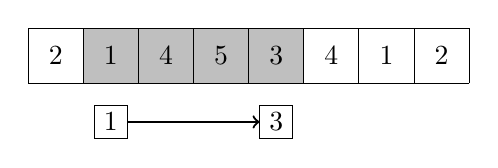
\begin{tikzpicture}[scale=0.7]
\fill[color=lightgray] (1,0) rectangle (5,1);
\draw (0,0) grid (8,1);

\node at (0.5,0.5) {$2$};
\node at (1.5,0.5) {$1$};
\node at (2.5,0.5) {$4$};
\node at (3.5,0.5) {$5$};
\node at (4.5,0.5) {$3$};
\node at (5.5,0.5) {$4$};
\node at (6.5,0.5) {$1$};
\node at (7.5,0.5) {$2$};

\draw (1.2,0.2-1.2) rectangle (1.8,0.8-1.2);
\draw (4.2,0.2-1.2) rectangle (4.8,0.8-1.2);

\node at (1.5,0.5-1.2) {$1$};
\node at (4.5,0.5-1.2) {$3$};

\draw[->,thick] (1.8,0.5-1.2) -- (4.2,0.5-1.2);
\end{tikzpicture}
\end{center}

Successivamente la finestra si muove ancora,
e l'elemento 1 non si trova più al suo interno.
Quindi, dopo che viene rimosso dalla coda,
il valore più piccolo diventa il 3,
inoltre viene aggiunto il nuovo valore 4.
\begin{center}
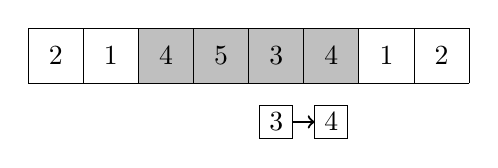
\begin{tikzpicture}[scale=0.7]
\fill[color=lightgray] (2,0) rectangle (6,1);
\draw (0,0) grid (8,1);

\node at (0.5,0.5) {$2$};
\node at (1.5,0.5) {$1$};
\node at (2.5,0.5) {$4$};
\node at (3.5,0.5) {$5$};
\node at (4.5,0.5) {$3$};
\node at (5.5,0.5) {$4$};
\node at (6.5,0.5) {$1$};
\node at (7.5,0.5) {$2$};

\draw (4.2,0.2-1.2) rectangle (4.8,0.8-1.2);
\draw (5.2,0.2-1.2) rectangle (5.8,0.8-1.2);

\node at (4.5,0.5-1.2) {$3$};
\node at (5.5,0.5-1.2) {$4$};

\draw[->,thick] (4.8,0.5-1.2) -- (5.2,0.5-1.2);
\end{tikzpicture}
\end{center}

Il nuovo elemento che a questo punto entrerà nella 
finestra è 1, che è più piccolo di tutti gli elementi
già presenti nella coda.
Verranno quindi rimossi tutti e solo l'1 rimarrà all'interno della
coda.
\begin{center}
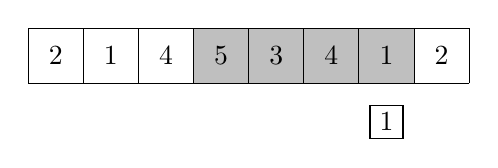
\begin{tikzpicture}[scale=0.7]
\fill[color=lightgray] (3,0) rectangle (7,1);
\draw (0,0) grid (8,1);

\node at (0.5,0.5) {$2$};
\node at (1.5,0.5) {$1$};
\node at (2.5,0.5) {$4$};
\node at (3.5,0.5) {$5$};
\node at (4.5,0.5) {$3$};
\node at (5.5,0.5) {$4$};
\node at (6.5,0.5) {$1$};
\node at (7.5,0.5) {$2$};

\draw (6.2,0.2-1.2) rectangle (6.8,0.8-1.2);

\node at (6.5,0.5-1.2) {$1$};
\end{tikzpicture}
\end{center}

Infine la finestra raggiungerà l'ultima posizione.
L'elemento 2 verrà aggiunto alla coda, 
ma il valore più piccolo rimarrà l'1.
\begin{center}
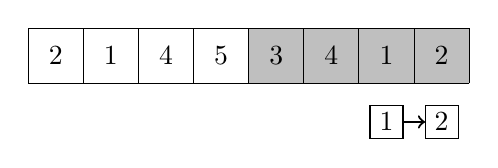
\begin{tikzpicture}[scale=0.7]
\fill[color=lightgray] (4,0) rectangle (8,1);
\draw (0,0) grid (8,1);

\node at (0.5,0.5) {$2$};
\node at (1.5,0.5) {$1$};
\node at (2.5,0.5) {$4$};
\node at (3.5,0.5) {$5$};
\node at (4.5,0.5) {$3$};
\node at (5.5,0.5) {$4$};
\node at (6.5,0.5) {$1$};
\node at (7.5,0.5) {$2$};

\draw (6.2,0.2-1.2) rectangle (6.8,0.8-1.2);
\draw (7.2,0.2-1.2) rectangle (7.8,0.8-1.2);

\node at (6.5,0.5-1.2) {$1$};
\node at (7.5,0.5-1.2) {$2$};

\draw[->,thick] (6.8,0.5-1.2) -- (7.2,0.5-1.2);
\end{tikzpicture}
\end{center}

Dal momento che ogni elemento dell'array
viene aggiunto alla coda esattamente una volta
e rimosso dalla coda al massimo una volta,
l'algoritmo ha una complessità di $O(n)$.



